\documentclass[12pt,a4paper]{article}
\usepackage[utf8]{inputenc}
\usepackage[spanish,es-tabla]{babel}
\usepackage{geometry}
\usepackage{graphicx}
\usepackage{multirow}
\usepackage{tabularx}
\usepackage{mathptmx}
\usepackage{fancyhdr}
\usepackage{array}
\usepackage[table]{xcolor}
\usepackage{titlesec}
\usepackage{setspace}
\usepackage{microtype}
\usepackage{lastpage}
\usepackage{booktabs}
\usepackage{enumitem}
\usepackage{amsmath}
\usepackage{amsfonts}
\usepackage{amssymb}
\usepackage{listings}

\lstset{
  basicstyle=\ttfamily\footnotesize,
  backgroundcolor=\color{gray!10},
  frame=single,
  breaklines=true,
  tabsize=2,
  showstringspaces=false
}

\graphicspath{{images/}{../images/}{./}}

\geometry{
    top=4.7cm,
    bottom=2.5cm,
    left=2.5cm,
    right=2.5cm,
    headheight=3.9cm,
    headsep=0.4cm
}

\setstretch{1.15}
\setlength{\parindent}{0pt}
\setlength{\parskip}{0.45em}
\setlength{\tabcolsep}{4pt}

\titleformat{\section}
  {\normalfont\fontsize{12}{14.5}\bfseries}{\thesection.}{0.6em}{\uppercase}
\titlespacing*{\section}
  {0pt}{1.8ex plus 0.4ex minus 0.2ex}{0.6ex plus 0.2ex}

\titleformat{\subsection}
  {\normalfont\fontsize{11.5}{13.5}\bfseries}{\thesubsection.}{0.5em}{}
\titlespacing*{\subsection}
  {0pt}{1.4ex plus 0.3ex minus 0.1ex}{0.4ex plus 0.1ex}

\titleformat{\subsubsection}
  {\normalfont\fontsize{10.5}{12.5}\bfseries\itshape}{\thesubsubsection.}{0.4em}{}
\titlespacing*{\subsubsection}
  {0pt}{1.1ex plus 0.2ex minus 0.1ex}{0.3ex plus 0.1ex}

\newcolumntype{Y}{>{\centering\arraybackslash}X}
\newcolumntype{L}{>{\raggedright\arraybackslash}X}
\newcolumntype{C}{>{\centering\arraybackslash}X}

\definecolor{headerred}{RGB}{180, 0, 0}
\definecolor{darkred}{RGB}{140, 0, 0}
\definecolor{lightgraybg}{RGB}{248, 248, 248}
\definecolor{tableheader}{RGB}{232, 238, 246}

\newcommand{\docCodigo}{TI-SIGE-ENT-S1-005}
\newcommand{\docVersion}{1.0}
\newcommand{\docProceso}{INGENIERÍA DE SOFTWARE / REGLAS DE NEGOCIO}
\newcommand{\docElaboracion}{20/08/2026}
\newcommand{\docRevision}{PENDIENTE DE REVISIÓN}
\newcommand{\docTitulo}{ESPECIFICACIÓN FORMAL DE REGLAS DE NEGOCIO Y VALIDATION GATES}
\newcommand{\docOrganizacion}{FACULTAD DE INGENIERÍA EN SISTEMAS, ELECTRÓNICA E INDUSTRIAL}
\newcommand{\docSubOrganizacion}{CARRERA DE INGENIERÍA DE SOFTWARE}

\newcommand{\encabezadofrecuente}{%
    \renewcommand{\arraystretch}{1.15}%
    \noindent\makebox[\textwidth][c]{%
    \begin{tabularx}{\textwidth}{|>{\centering\arraybackslash}m{2.8cm}|Y|>{\centering\arraybackslash}m{4.8cm}|}
        \hline
        \multirow{4}{2.8cm}{\centering\raisebox{-1.15cm}{
\includegraphics[width=2.5cm,height=2.0cm,keepaspectratio]{images/logo.png}}}
        & \textbf{\fontsize{9}{11}\selectfont \docOrganizacion} 
        & \textbf{\fontsize{8}{10}\selectfont CÓDIGO:} \fontsize{8}{10}\selectfont \docCodigo \\
        \cline{3-3}
        & \textbf{\fontsize{8.5}{10.5}\selectfont \docSubOrganizacion} 
        & \textbf{\fontsize{8}{10}\selectfont VERSIÓN:} \fontsize{8}{10}\selectfont \docVersion \\
        \cline{2-3}
        & \textbf{\fontsize{8}{10}\selectfont PROCESO:} \fontsize{8}{10}\selectfont \docProceso 
        & \textbf{\fontsize{8}{10}\selectfont ELABORACIÓN:} \fontsize{8}{10}\selectfont \docElaboracion \\
        \cline{2-3}
        & \textbf{\fontsize{8.5}{10.5}\selectfont \docTitulo} 
        & \textbf{\fontsize{8}{10}\selectfont ÚLTIMA REVISIÓN:} \fontsize{8}{10}\selectfont \textbf{\textcolor{darkred}{\docRevision}} \\
        \hline
    \end{tabularx}%
    }%
}

\pagestyle{fancy}
\fancyhf{}
\fancyhead[C]{\encabezadofrecuente}
\fancyfoot[C]{\fontsize{10}{12}\selectfont Página \thepage\ de \pageref{LastPage}}
\renewcommand{\headrulewidth}{0pt}

\begin{document}

\section{Título}
\textbf{Denominación del Entregable:} Catálogo de Reglas de Negocio Institucionales y Motor de Validation Gates (EDT 1.5)

\vspace{0.15cm}
\noindent
\textbf{Ficha Técnica de Identificación:}
\begin{itemize}[leftmargin=1.5em, itemsep=1.5pt, topsep=1.5pt]
    \item \textbf{Código Documental:} \docCodigo \quad | \quad \textbf{Versión:} \docVersion
    \item \textbf{Institución:} Universidad Técnica de Ambato (UTA) -- FISEI
    \item \textbf{Carrera:} Ingeniería de Software (Séptimo Semestre "A")
    \item \textbf{Módulo Académico:} Gestión de Proyectos de Software
    \item \textbf{Docente Tutor:} Ing. Paulo Torres
    \item \textbf{Fecha de Elaboración:} \docElaboracion \quad | \quad \textbf{Estado:} \textbf{\textcolor{darkred}{En Elaboración / Pendiente de Revisión}}
    \item \textbf{Período de Ejecución:} Semana 1 (20/08/2026 al 22/08/2026)
    \item \textbf{Responsables:} Steeven Toala (Líder / Arquitecto) y Nixon Hurtado (Backend / DBA)
\end{itemize}

\section{Introducción}
La confiabilidad y rigor del sistema \textbf{SIGE} radica en su capacidad para garantizar el cumplimiento normativo institucional del Sistema de Gestión de la Calidad (SGC). En este documento se especifican formalmente las \textbf{Reglas de Negocio (RN)} y la arquitectura de compuertas secuenciales (\textbf{Validation Gates}) implementadas de forma determinista en cliente (React + Zod) y servidor (.NET 9 + FluentValidation) que impiden el avance, guardado o envío de documentos con inconsistencias aritméticas o documentales.

\section{Concepto y Arquitectura de Validation Gates}
Los \textbf{Validation Gates} (Compuertas de Validación Deterministas) evalúan precondiciones y postcondiciones en cada transición de estado:
\begin{itemize}[leftmargin=1.5em, itemsep=2pt]
    \item \textbf{Gate 1 (Matriz Completa):} Comprueba que cada fila de la matriz de actividades contenga todos los campos obligatorios antes de permitir la adición de una nueva fila o el avance de fase.
    \item \textbf{Gate 2 (Evidencias en MinIO):} Bloquea el envío al comité si existen actividades con porcentaje de avance mayor al $0\%$ sin archivos probatorios cargados en MinIO.
    \item \textbf{Gate 3 (Suma de Ponderación = 100\%):} Verifica que la sumatoria total de ponderaciones de las actividades equivalga estrictamente al $100.0\%$.
    \item \textbf{Gate 4 (Firma Previa Válida en Cascada):} Impide que una instancia superior (Coordinador de Área o Carrera) estampe su firma electrónica si la instancia predecesora no ha firmado válidamente.
\end{itemize}

\begin{figure}[htbp]
    \centering
    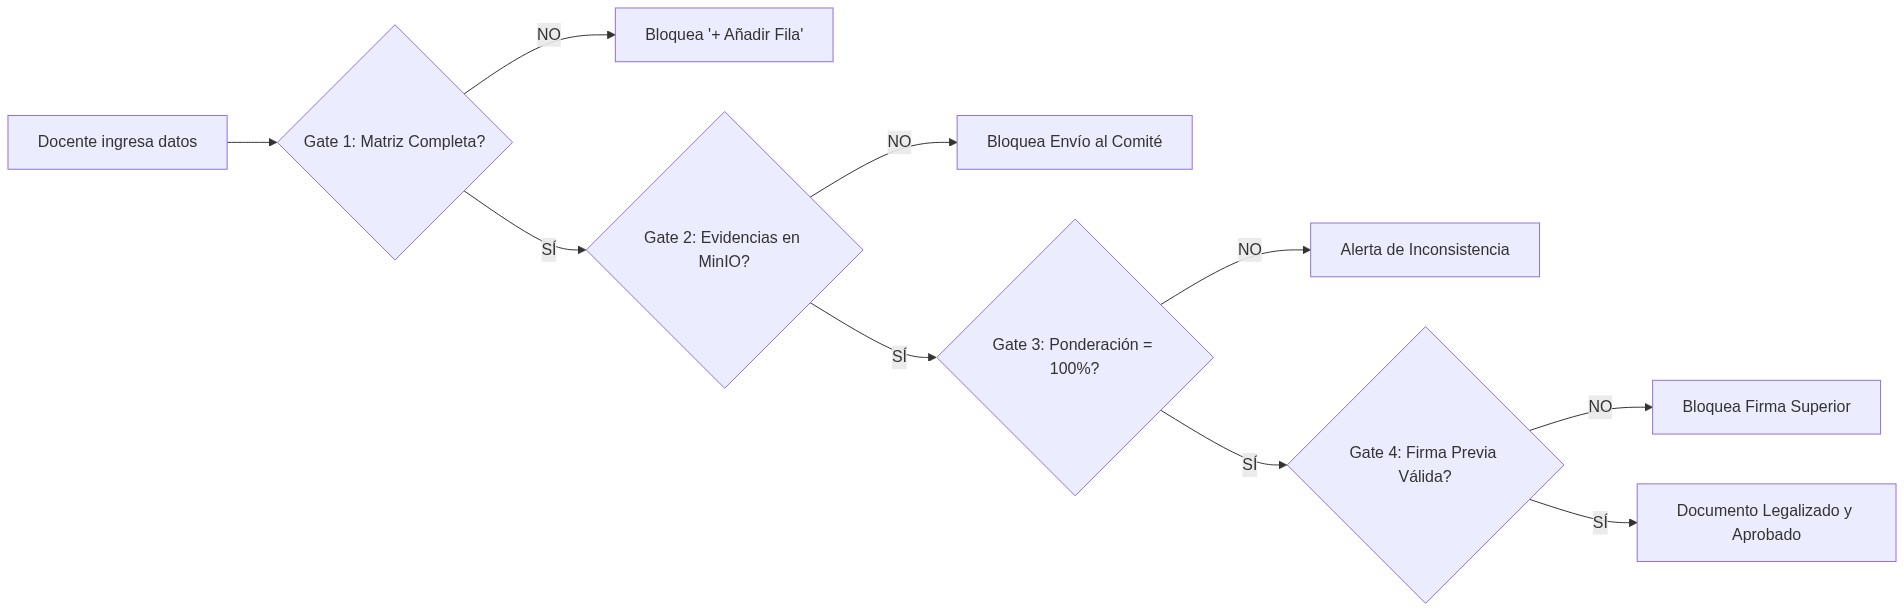
\includegraphics[width=0.88\textwidth,height=5.2cm,keepaspectratio]{images/s1_05_validation_gates.png}
    \caption{Arquitectura Secuencial de Validation Gates en el Flujo Documental SIGE.}
    \label{fig:s1_05_vg}
\end{figure}

\section{Especificación Detallada de Reglas de Negocio}

\subsection{RN-01: Fechas Autogeneradas e Inmutables}
\begin{itemize}[leftmargin=1.5em, itemsep=1.5pt]
    \item \textbf{Descripción:} Las fechas de emisión, registro y marcas temporales de cambios son generadas exclusivamente por el reloj del servidor (\texttt{DateTime.UtcNow}).
    \item \textbf{Comportamiento:} En la interfaz de usuario, estos campos se renderizan en modo solo lectura (\texttt{readonly}). No se acepta ningún valor de fecha de emisión enviado desde el cuerpo de la petición HTTP (\textit{Payload tampering protection}).
\end{itemize}

\subsection{RN-02: Detección Automática del Período Académico}
\begin{itemize}[leftmargin=1.5em, itemsep=1.5pt]
    \item \textbf{Descripción:} El sistema identifica el período académico oficial vigente según el calendario institucional:
    \[
    \text{Período} = \begin{cases} 
    \text{Julio } [A\tilde{n}o] \text{ -- Diciembre } [A\tilde{n}o] & \text{si Mes} \in [7, 12] \\ 
    \text{Enero } [A\tilde{n}o] \text{ -- Junio } [A\tilde{n}o] & \text{si Mes} \in [1, 6] 
    \end{cases}
    \]
    \item \textbf{Comportamiento:} El usuario no puede modificar el período para evitar asimetrías en las auditorías semestrales.
\end{itemize}

\subsection{RN-03: Llenado Estricto de Matriz Fila por Fila}
\begin{itemize}[leftmargin=1.5em, itemsep=1.5pt]
    \item \textbf{En el Plan de Trabajo (\texttt{UTA-SGC-A-2-1-P7-T1}):} Para habilitar la fila $N+1$, la fila $N$ debe satisfacer la condición lógica:
    \[
    \text{FilaVálida}(N) = (\text{Actividad} \neq \emptyset) \land (\text{Desde} \le \text{Hasta}) \land (\text{Responsable} \neq \emptyset) \land (\text{Recursos} \neq \emptyset) \land (\text{Medios} \neq \emptyset)
    \]
    \item \textbf{En el Informe de Cumplimiento (\texttt{UTA-SGC-A-2-1-P7-T2}):}
    \[
    \text{FilaInformeVálida}(N) = (\text{Actividad} \neq \emptyset) \land (\text{MedioVerificación} \neq \emptyset) \land (\text{Avance} \in [0, 100]) \land (\text{Avance} < 100 \implies \text{Observación} \neq \emptyset)
    \]
    \item \textbf{Comportamiento:} El botón \textbf{\texttt{[+ Añadir Fila]}} permanece deshabilitado hasta que la condición se evalúa como verdadera.
\end{itemize}

\subsection{RN-04: Obligatoriedad de Medios de Verificación en MinIO S3}
\begin{itemize}[leftmargin=1.5em, itemsep=1.5pt]
    \item \textbf{Descripción:} Ninguna actividad puede registrar un avance porcentual superior al $0\%$ si no tiene adjunto al menos un archivo de verificación cargado en el bucket de MinIO.
    \item \textbf{Validación Backend (FluentValidation en C\#):}
\end{itemize}
\begin{lstlisting}[language={[Sharp]C}]
RuleFor(a => a.Evidencias)
    .NotEmpty()
    .When(a => a.PorcentajeAvance > 0)
    .WithMessage("Toda actividad con avance mayor a 0% requiere al menos una evidencia cargada en MinIO.");
\end{lstlisting}

\subsection{RN-05: Justificación Obligatoria de Desvío ($< 100\%$)}
\begin{itemize}[leftmargin=1.5em, itemsep=1.5pt]
    \item \textbf{Descripción:} Toda actividad cuyo avance no alcance el $100\%$ debe justificar la causa del retraso o reprogramación en el campo de observaciones.
    \item \textbf{Validación Backend (FluentValidation en C\#):}
\end{itemize}
\begin{lstlisting}[language={[Sharp]C}]
RuleFor(a => a.Observaciones)
    .NotEmpty()
    .MinimumLength(10)
    .When(a => a.PorcentajeAvance < 100)
    .WithMessage("Las actividades con avance menor al 100% deben incluir una justificación de desvío de al menos 10 caracteres.");
\end{lstlisting}

\subsection{RN-06: Validación de Suma Ponderada Total ($100.0\%$)}
\begin{itemize}[leftmargin=1.5em, itemsep=1.5pt]
    \item \textbf{Descripción:} La sumatoria de las ponderaciones asignadas a las actividades del Plan de Trabajo debe totalizar exactamente el $100\%$:
    \[
    \sum_{i=1}^{k} \text{Ponderación}_i = 100.0\%
    \]
\end{itemize}

\subsection{RN-07: Flujo Secuencial de Firmas sin Omisión de Pasos}
\begin{itemize}[leftmargin=1.5em, itemsep=1.5pt]
    \item \textbf{Descripción:} El orden de firmas en cascada es estricto e inviolable:
    \[
    \text{Firma 1 (Docente Elaborador)} \longrightarrow \text{Firma 2 (Coordinador de Área)} \longrightarrow \text{Firma 3 (Coordinador de Carrera)}
    \]
    \item \textbf{Comportamiento:} El endpoint de firma del Revisor rechaza solicitudes si no existe la firma del Elaborador. El endpoint del Validador rechaza si falta la del Revisor.
\end{itemize}

\subsection{RN-08: Gestión de Rechazos y Versionado Automático}
\begin{itemize}[leftmargin=1.5em, itemsep=1.5pt]
    \item \textbf{Descripción:} Al emitir un dictamen de rechazo o devolución por parte del Revisor o Validador:
    \begin{enumerate}[leftmargin=1.5em, itemsep=1pt]
        \item Es obligatorio registrar la observación granular justificando el rechazo.
        \item El estado del documento cambia automáticamente a \texttt{OBSERVADO\_DEVUELTO}.
        \item El sistema crea una nueva entrada en el historial incrementando la versión (\texttt{V01} $\rightarrow$ \texttt{V02}).
        \item Se notifica automáticamente al docente elaborador por correo institucional (SMTP).
    \end{enumerate}
\end{itemize}

\subsection{RN-09: Registro Inmutable de Auditoría}
\begin{itemize}[leftmargin=1.5em, itemsep=1.5pt]
    \item \textbf{Descripción:} Toda transición de estado, firmado digital o carga de evidencias genera un registro en la tabla de auditoría con: \texttt{UsuarioId}, \texttt{Rol}, \texttt{AccionRealizada}, \texttt{DireccionIP}, \texttt{Timestamp} y \texttt{HashSHA256} del contenido generado.
\end{itemize}

\vspace{0.3cm}

% =============================================================
% FIRMAS DE RESPONSABILIDAD
% =============================================================
\section{Firmas de Responsabilidad}

\noindent
\renewcommand{\arraystretch}{1.2}
\begin{tabularx}{\textwidth}{|>{\raggedright\arraybackslash}m{2.9cm}|>{\raggedright\arraybackslash}X|>{\centering\arraybackslash}m{4.6cm}|>{\centering\arraybackslash}m{2.3cm}|}
    \hline
    \rowcolor{headerred}
    \textcolor{white}{\textbf{ACCIÓN}} & \textcolor{white}{\textbf{NOMBRE Y CARGO}} & \textcolor{white}{\textbf{FIRMA}} & \textcolor{white}{\textbf{FECHA}} \\
    \hline
    \textbf{Elaborado por:} & Steeven Toala\newline \textit{Líder de Proyecto / Arquitecto Software} & \parbox[c]{4.4cm}{\centering\vspace{4pt}
\includegraphics[height=1.5cm,width=4.0cm,keepaspectratio]{images/firma_steveen.png}\vspace{4pt}} & 20/08/2026 \\
    \hline
    \textbf{Revisado por:} & Steeven Toala\newline \textit{Líder de Proyecto / Arquitecto Software} & \parbox[c]{4.4cm}{\centering\vspace{10pt}\textbf{\textcolor{gray!80}{\scriptsize [ PENDIENTE DE REVISIÓN ]}}\vspace{10pt}} & \textbf{\textcolor{gray!90}{Pendiente}} \\
    \hline
    \textbf{Aprobado por:} & Ing. Paulo Torres\newline \textit{Docente Tutor - Gestión Proyectos Software} & \parbox[c]{4.4cm}{\centering\vspace{10pt}\textbf{\textcolor{gray!80}{\scriptsize [ PENDIENTE DE APROBACIÓN ]}}\vspace{10pt}} & \textbf{\textcolor{gray!90}{Pendiente}} \\
    \hline
\end{tabularx}

\vspace{0.4cm}

% =============================================================
% CONTROL DE CAMBIOS
% =============================================================
\section{Control de Cambios}

\noindent
\renewcommand{\arraystretch}{1.2}
\begin{tabularx}{\textwidth}{|>{\hsize=0.45\hsize\centering\arraybackslash}X|>{\hsize=1.55\hsize\raggedright\arraybackslash}X|>{\hsize=1.2\hsize\raggedright\arraybackslash}X|>{\hsize=0.8\hsize\centering\arraybackslash}X|}
    \hline
    \rowcolor{gray!20}
    \textbf{Versión} & \textbf{Descripción del cambio} & \textbf{Responsable del cambio} & \textbf{Fecha de aprobación} \\
    \hline
    1.0 & Especificación formal de reglas de negocio RN-01 a RN-09 y motor de validation gates / Pendiente de revisión & Steeven Toala & \textbf{\textcolor{gray!90}{Pendiente de Revisión}} \\
    \hline
\end{tabularx}

\vspace{0.4cm}

\section{Anexos}
\subsection*{Anexo 1: Pipeline Behaviors de MediatR para Validation Gates}
Patrón de intercepción en ASP.NET Core que evalúa las reglas de validación en tiempo de compilación y ejecución antes de persistir los cambios en PostgreSQL.

\end{document}
